\begin{figure}[H]
  \caption{Ubicacción de estaciones de trasporte en Bogota, D.C}\label{fig:hists}
  \hspace{-2cm} % Ajusta el espacio horizontal entre la figura y el margen izquierdo
  \subfloat[Ubicación de estaciones transmilenio\label{subfiga:Transmi}]{
    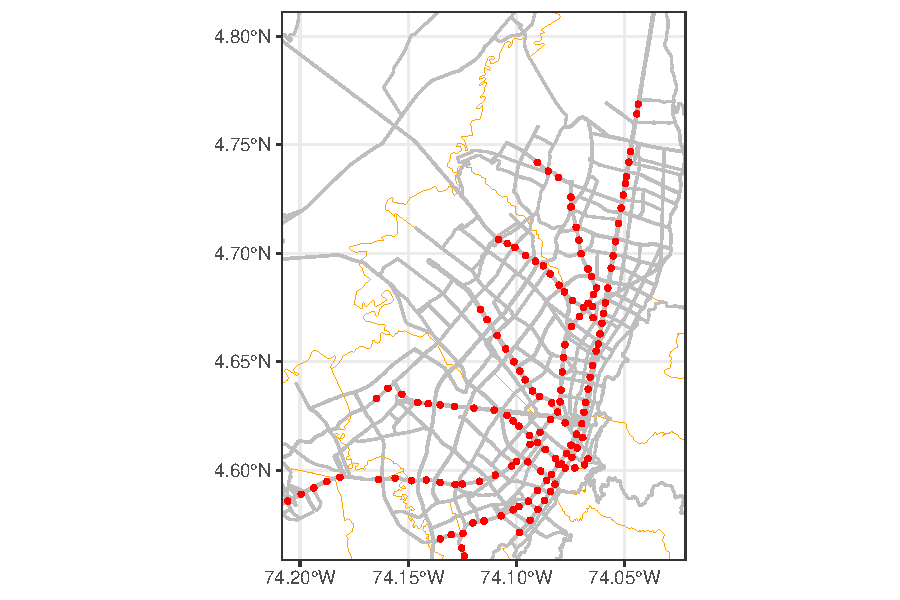
\includegraphics[width=0.7\textwidth, align=l]{graficos/mapatransmi.pdf}}
  \hspace{-2.8cm} % Ajusta el espacio horizontal entre las subfiguras
  \subfloat[Ubicación de estaciones de SITP\label{subfigb:sipt}]{
    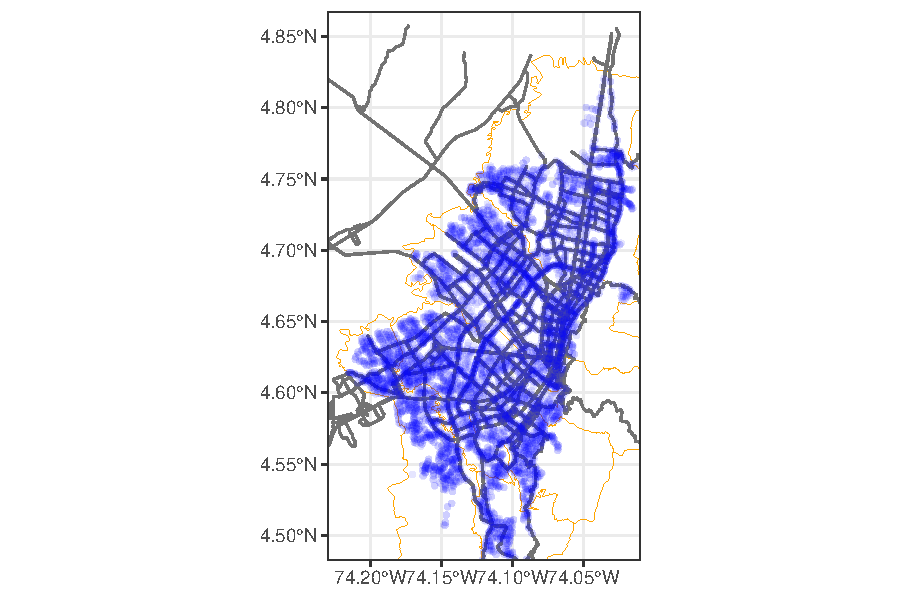
\includegraphics[width=0.7\textwidth, align=l]{graficos/mapasitp.pdf}}
  \begin{center}
    \footnotesize{\textbf{Fuente:} Elaboración propia con train.csv, 2024.}
  \end{center}
\end{figure}
